\section{rSLA runtime architecture and implementation }

The rSLA Service is designed to be run either by a service provider, a customer, or a third party such as a service integrator.  The following section  explains the components constituting the rSLA service and its interaction with xlets.  

\begin{figure}[htb]
\centering
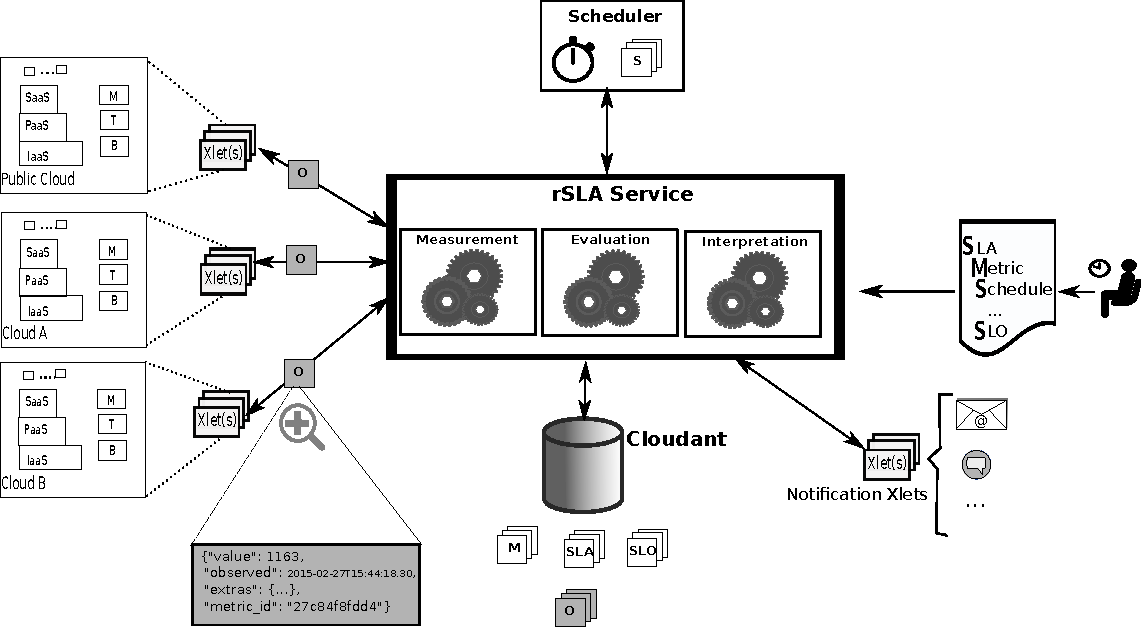
\includegraphics[width=\textwidth]{pics/runtime.pdf}
\caption{\label{fig:runtime} rSLA runtime}
\end{figure}


\subsection{rSLA service}
The rSLA service is a Ruby Sinatra application, a given because it is a Ruby DSL. It is implemented to run on a Cloud Foundry PaaS. We have chosen IBM's Bluemix Cloud Foundry application. It offers different REST interfaces that allow the management of the life cycle of an SLA described using our DSL.

The rSLA service exposes a set life cycle management functions to its user, in particular to create, activate, deactivate and remove SLSs. At the reception of a new SLA, the rSLA Service interprets the file and creates a set of objects. The new objects are persisted in a Cloudant no-SQL database service using a CouchRest Model.

On the {\em activation} of an SLA, the rSLA Service orchestrates all the needed operations to activate and manage the SLA life cycle. It starts by scheduling data collection for base 
metrics with the rSLA scheduler service, which is a companion service to the rSLA application itself. As shown in Figure~\ref{fig:runtime}, based on the defined schedules, the scheduler triggers the needed rSLA Service interfaces. This latter will then invoke the 
monitoring Xlets to collect new observations for the related base metrics. Afterwards, the observations are persisted in Cloudant. Observations are  JSON structures returned by monitoring xlets that contain the metric value requested, a time stamp, and any additional information that might be of relevance understanding the metric. For example, in case of our provisioning processes, in addition to the provisioning time as the value of the metric it may be interesting to know which particular server has been provisioned if a particular process takes longer than expected.

Similarly, according to the schedule of an SLO, the 
Scheduler triggers an rSLA Service interface for SLO evaluation. The rSLA service will then retrieve the data related to the specific SLO, reify the corresponding metrics as Ruby objects and then evaluate the expressions of the SLO, precondition and objective. As an optimization step, this evaluation may use the  map-reduce functions offered by Cloudant to delegate  possible parallel processings to Cloudant and benefit from its efficiency.

Afterwards, the rSLA Service generates JSON notifications representing the results of the evaluation. These notifications are sent to the Notification Xlet for formatting and reporting to the client.   

\subsection{rSLA Xlets}

As described previously in this paper, xlets offer a standard interface for monitoring and notification as a generic REST API, abstracting from the heterogeneity of different service interfaces. In our architecture, xlets are services on Bluemix.
 An Xlet is customized according to its role in the overall system. As shown in Figure~\ref{fig:xlet}, each Xlet provides three 
interfaces:

\begin{itemize}
 \item \emph{CFBrokerInterface}: Since the Xlets are provided as services by Bluemix , they need to offer this generic interface that describes exactly how to provision the 
service, how to unprovision it, how to bind the service to a given application and how to unbind it. 
\item  \emph{ConfigurationInterface}: In order to ensure multi-tenancy and customization of an Xlet, it must offer an interface to configure its tenancy. This interface could offer other functionalities of customization, e.g., to configure the access credentials for Cloud resources.
\item  \emph{RuntimeInterface}: This interface provides the main business of the xlet. It describes the specific functionalities to be offered by the application instance (e.g., monitoring services, reporting services). 
\end{itemize}
\begin{figure}[H]
\centering
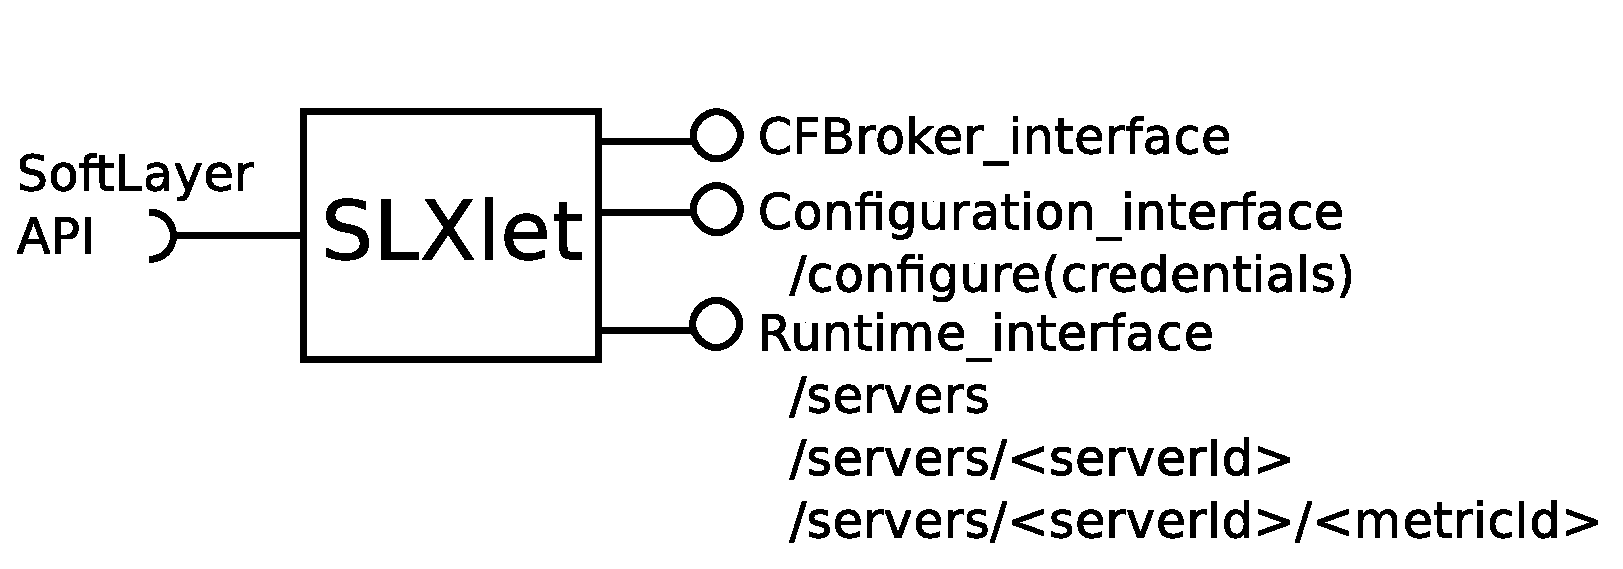
\includegraphics[width=0.6\textwidth]{pics/SLXlet}
\caption{\label{fig:xlet} Xlet interface design}
\end{figure}

All xlets observe the same architecture but differ in their implementations from one use case to another. The runtime interface of the monitoring Xlets are in line with the DMTF Cloud Infrastructure Management Model (CIMI, CITATION). They allow collecting monitoring data for a specific type of resources with different granularities. For example, 
Figure~\ref{fig:xlet} shows a SoftLayer specific Xlet. The SLXlet allows to get monitoring data of SoftLayer-provisioned servers for a given account. The account credentials are 
passed to the Xlet in the configuration phase through the Configuration interface. Afterwards, the runtime interface of the Xlet can be used to get the list of servers, the list 
of metrics for a given server, or the value for a given metric for a specific server.


Using Bluemix as xlet platform has  advantageous characteristics: {\em scalability} is inherited from the scalability of Bluemix environment. Since the xlet can be provisioned as an application or a service within 
Bluemix, it is easy to scale it horizontally to cope with the work load by adding or removing new instances.
All Xlets have a common and generic core code that often allow the easy {\em reusability} with minor modifications for specific use cases.
{\em Managing} xlets is handled to Bluemix, the management here includes provisioning, deprovisioning, binding and unbinding xlets to the rSLA service.
Xlets can be integrated {\em flexibly} using Bluemix services and can be provisioned using different plans, e.g., shared or dedicated. 


\subsection{Case Study}

We have conducted a pilot of the rSLA service to support the management of cloud services used by an existing customer. In one agreement, the  customer migrated a workload from a customer-owned, on-premise data center environment to the IBM cloud.  Along with the move, the customer required the monitoring of seven custom SLOs that had never been offered previously by the service provider in the cloud.

Each of the seven  SLOs consist of one base metric and one service level objective, with multiple composite metrics used to aggregate to level needed by the SLOs. The rSLA document has been defined based on the written agreement with the customer and discussions with the client. The rSLA was submitted and  executed by the rSLA service to activate and initiate the measurement of the involved base metrics. The rSLA service monitors, measures, evaluates and reports the service level status of the seven involved SLOs on a daily basis to the customer, resulting in about 100MB/month in observation data.

We developed three different xlets to monitor various aspects of the service such as network status and provisioning process times, as well as one xlet for email notification. Overall, it took 3 weeks from first contact with the project team to the start of monitoring. This included the development of the specific xlets, the definition of the SLA document, and obtaining the access keys to the client's Cloud service API. This is much faster than a traditional integration to an enterprise SLA management system. In a future scenario another user of the rSLA can re-use the xlets and the remaining effort only comprises the writing of the SLA document and obtaining the API keys for monitoring xlet configuration, which may be as little as a number of hours or a day.



